\documentclass[12pt,a4paper]{article}

\usepackage[a4paper,margin=1.65cm]{geometry}
\usepackage{amsmath,amssymb}
\usepackage{graphicx}
\usepackage{booktabs}
\usepackage{array}
\usepackage{xcolor}
\usepackage{hyperref}
\usepackage{float}
\usepackage{caption}
\usepackage{subcaption}
\usepackage{parskip}
\usepackage{titlesec}
\usepackage{fancyhdr}
\usepackage{microtype}
\usepackage{mdframed}

\definecolor{iiscblue}{RGB}{0,50,120}
\definecolor{resultsbox}{RGB}{244,248,252}

\hypersetup{
  colorlinks=true,
  linkcolor=iiscblue,
  urlcolor=iiscblue,
  citecolor=iiscblue
}

\titleformat{\section}{\large\bfseries\color{iiscblue}}{}{0em}{}[\titlerule]
\titleformat{\subsection}{\normalsize\bfseries\color{iiscblue!85}}{}{0em}{}
\titlespacing{\section}{0pt}{8pt}{4pt}
\titlespacing{\subsection}{0pt}{5pt}{2pt}

\pagestyle{fancy}
\fancyhf{}
\fancyhead[L]{\small\textcolor{iiscblue}{\textbf{PRNN Assignment 2}}}
\fancyhead[R]{\small\textcolor{gray}{Bitupan Arandhara}}
\fancyfoot[C]{\small\textcolor{gray}{\thepage}}
\renewcommand{\headrulewidth}{0.4pt}
\renewcommand{\headrule}{\hbox to\headwidth{\color{iiscblue}\leaders\hrule height \headrulewidth\hfill}}

\newmdenv[
  backgroundcolor=resultsbox,
  linecolor=iiscblue,
  linewidth=0.8pt,
  leftmargin=0pt,
  rightmargin=0pt,
  innerleftmargin=8pt,
  innerrightmargin=8pt,
  innertopmargin=5pt,
  innerbottommargin=5pt
]{resultbox}

\graphicspath{{report_assets/}}

\begin{document}

\begin{center}
  {\LARGE\bfseries\color{iiscblue} Pattern Recognition and Neural Networks}\\[4pt]
  {\large Assignment 2}\\[4pt]
  {\normalsize Bitupan Arandhara \quad SR No: 04-03-00-10-22-25-1-25910}\\[3pt]
  \textcolor{gray}{\rule{0.85\linewidth}{0.4pt}}
\end{center}

\section{Phase 1: MLP Baseline \& Gradient Flow}

\subsection{1.1 Flattened Temporal MLP (Regression)}
\vspace{6pt}
\begin{resultbox}
Delhi AQI was loaded from \texttt{delhi\_aqi.csv} after dropping the date column. Each sample uses the previous $72$ hours of all $8$ features, flattened to a $576$-dimensional vector, to predict $\mathrm{PM}_{2.5}$ at $t+24$.

The implemented regressor is a 3-layer MLP,
\[
f(x)=W_3\,\phi\!\left(W_2\,\phi\!\left(W_1x+b_1\right)+b_2\right)+b_3,
\]
with hidden dimensions $256$ and ReLU activations.  \\ 
The MSE on the test set is \textbf{1.1314}.

\begin{figure}[H]
  \centering
  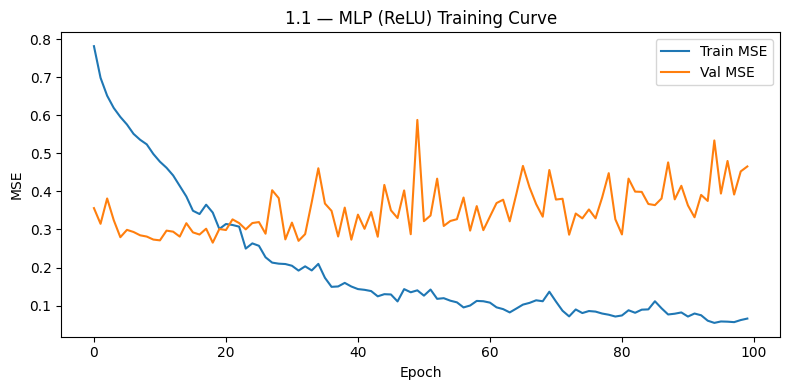
\includegraphics[width=0.54\linewidth]{q1_1_mlp_learning_curve.png}
  \caption{Training and validation MSE for the MLP.}
\end{figure}
\end{resultbox}

\subsection{1.2 The Vanishing Gradient Proof}
\vspace{6pt}
\begin{resultbox}
The same architecture was re-initialized with Sigmoid activations and backward hooks were used to record weight-gradient $\ell_2$ norms during the first epoch. Over the recorded $205$ batches, the mean gradient norms were:
\[
\|\nabla W_1\|_2 = 0.262829,\qquad
\|\nabla W_2\|_2 = 0.886609,\qquad
\|\nabla W_3\|_2 = 6.380196.
\]
The gradient decays in the initial layers.

\begin{figure}[H]
  \centering
  \begin{subfigure}[b]{0.63\linewidth}
    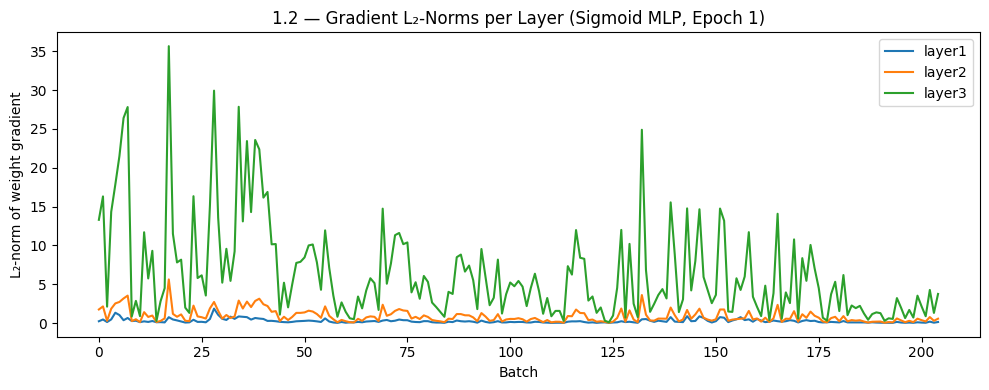
\includegraphics[width=\linewidth]{q1_2_sigmoid_gradients.png}
    \caption{Per-batch gradient norms.}
  \end{subfigure}
  \hfill
  \begin{subfigure}[b]{0.31\linewidth}
    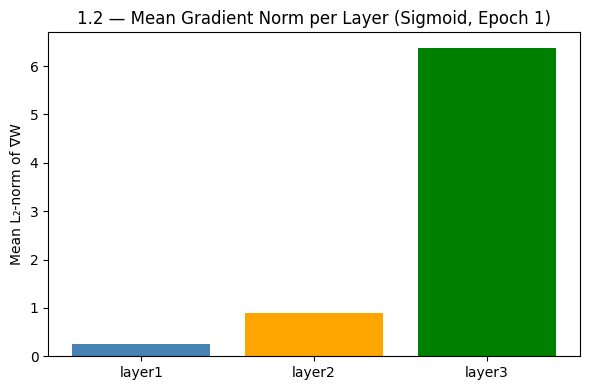
\includegraphics[width=\linewidth]{q1_2_sigmoid_mean_gradients.png}
    \caption{Layerwise means.}
  \end{subfigure}
  \caption{Gradient measurements for the Sigmoid MLP.}
\end{figure}
\end{resultbox}

\subsection{1.3 Imbalanced Threshold Classification}
\vspace{6pt}
\begin{resultbox}
The target variable PM2.5 was converted into a  binary classification task: 1 if $\mathrm{PM}_{2.5}>200$, else 0. The training split contains $5398$ positives out of $13076$ samples ($41.3\%$), giving \texttt{pos\_weight} $=1.42$. Two 3-layer classifiers were trained:
\begin{itemize}
  \item Model A: \texttt{BCELoss}.
  \item Model B: \texttt{BCEWithLogitsLoss} with \texttt{pos\_weight}.
\end{itemize}
The average Precision on the test set was \textbf{0.7838} for Model A and \textbf{0.7890} for Model B.

\begin{figure}[H]
  \centering
  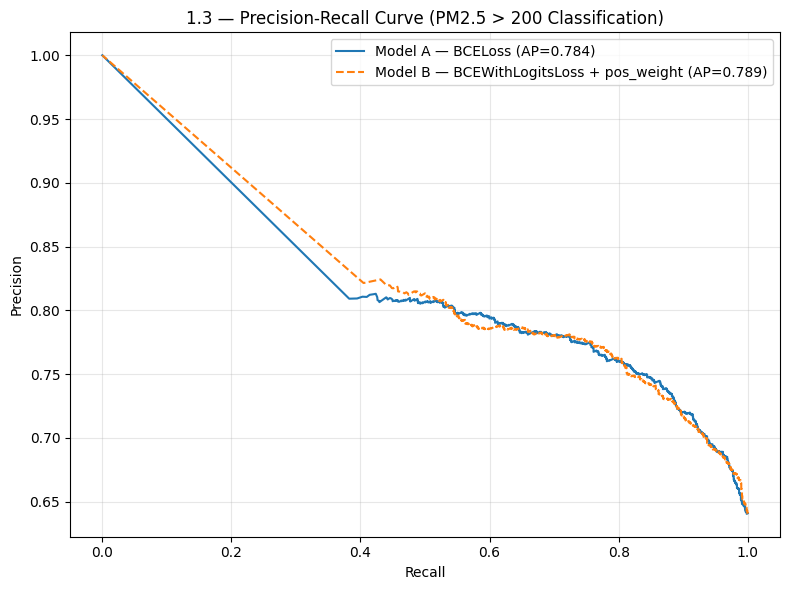
\includegraphics[width=0.52\linewidth]{q1_3_pr_curve.png}
  \caption{Precision--Recall curves for the two binary classifiers.}
\end{figure}
\end{resultbox}


\section{Phase 2: CNNs \& Spatial Hierarchies}

\subsection{2.4 CNN from Scratch \& Receptive Fields}
\vspace{6pt}
\begin{resultbox}
The PlantVillage classifier uses three convolutional blocks:
\[
\text{Conv1}(3\!\to\!8)\rightarrow\text{Pool1}\rightarrow
\text{Conv2}(8\!\to\!16)\rightarrow\text{Pool2}\rightarrow
\text{Conv3}(16\!\to\!32)\rightarrow\text{Pool3},
\]
followed by a linear head $8192 \rightarrow 256 \rightarrow 38$. Images are resized to $128\times128$. The theoretical receptive field of a single activation in the final feature map is \textbf{$22\times22$ pixels}. The test accuracy: \textbf{91.94\%} .
\end{resultbox}

\subsection{2.5 CNN Regression Head}
\vspace{6pt}
\begin{resultbox}
Modified the CNN architecture to perform regression:
\[
8192 \rightarrow 256 \rightarrow 64 \rightarrow 1,
\]
and a final Sigmoid output.
% The continuous severity target is synthesized in code: healthy images are assigned $0$, while diseased images receive a random value drawn uniformly from $[0.2,0.9]$. Dataset sizes are train $=38013$, val $=8145$, test $=8147$. 
The test MAE is \textbf{0.1371}.
\end{resultbox}

\subsection{2.6 Translation Invariance}
\vspace{6pt}
\begin{resultbox}
Accuracy on unshifted test images: \textbf{94.00\%}. \\
Accuracy on the same test images after pixel shifting: \textbf{90.00\%} (a \textbf{4.00\%} drop).\\
The reason for this performance drop is because max-pooling provides only local translation invariance. This invariance is limited to shifts smaller than the pooling stride. For a shift of 5 pixels:
 \begin{itemize}
     \item After three max-pool layers each with stride 2, the effective stride is $2^3 = 8$.
     \item A 5-pixel shift at the input level changes which values land in each pooling window. 
     \item The boundary between pooling windows shifts, so different feature values are selected by the max operation, due to which the activations in the final feature map changes and networks accuracy drops.
 \end{itemize}
 
\end{resultbox}

\section{Phase 3: RNNs \& Sequential Memory}

\subsection{3.7 Vanilla RNN from scratch}
\vspace{6pt}
\begin{resultbox}
% The RNN is implemented as
% \[
% h_t = \tanh(W_x x_t + W_h h_{t-1}), \qquad
% \hat{y} = W_y h_T,
% \]
% with a learned input projection, recurrent projection, and output layer. On the Delhi AQI single-step regression task, early stopping selected the best validation loss \textbf{0.2412}; the reported test MSE is \textbf{0.9237}.
Trained the Vanilla RNN model on the 72-hour historical sequences to predict the continuous PM2.5 value. \\
MSE on the test set: \textbf{0.9237}.
\end{resultbox}

\subsection{3.8 BPTT Decay}
\vspace{6pt}
\begin{resultbox}
% For a length-$100$ synthetic sequence, the notebook records the hidden-state gradient norms
% \[
% \left\|\frac{\partial \mathcal{L}}{\partial h_{100}}\right\| = 4.71\times 10^{-1},\quad
% \left\|\frac{\partial \mathcal{L}}{\partial h_{50}}\right\| = 6.76\times 10^{-21},\quad
% \left\|\frac{\partial \mathcal{L}}{\partial h_{0}}\right\| = 0.
% \]
\begin{center}
\setlength{\tabcolsep}{3pt} % Adjust this value as needed
\begin{tabular}{lc}
\toprule
\multicolumn{2}{l}{Gradient of the loss w.r.t. the hidden state for RNN} \\
\midrule
t = 100 & $4.71\times 10^{-1}$ \\
t = 50  & $6.76\times 10^{-21}$ \\
t = 0   & 0 \\
\bottomrule
\end{tabular}
\end{center}

\end{resultbox}

\subsection{3.9 Exploding gradients}
\vspace{6pt}
\begin{resultbox}
The largest singular value of the weight matrix is \textbf{1.1760}. The observed value is greater than $1$.
\end{resultbox}

\section{Phase 4: LSTMs, GRUs \& Context}

\subsection{4.10 LSTM Gradient Rescue}
\vspace{6pt}
\begin{resultbox}
% The LSTM experiment repeats the length-$100$ gradient measurement with an untrained \texttt{nn.LSTM}. The measured norms are
% \[
% \left\|\frac{\partial \mathcal{L}}{\partial h_{100}}\right\| = 7.78\times 10^{-2},\quad
% \left\|\frac{\partial \mathcal{L}}{\partial h_{50}}\right\| = 3.96\times 10^{-13},\quad
% \left\|\frac{\partial \mathcal{L}}{\partial h_{0}}\right\| = 0.
% \]

\begin{center}
\setlength{\tabcolsep}{3pt} % Adjust this value as needed
\begin{tabular}{lc}
\toprule
\multicolumn{2}{l}{Gradient of the loss w.r.t. the hidden state for LSTM} \\
\midrule
t = 100 & $7.78\times 10^{-2}$ \\
t = 50  & $3.96\times 10^{-13}}$ \\
t = 0   & 0 \\
\bottomrule
\end{tabular}
\end{center}


\begin{figure}[H]
  \centering
  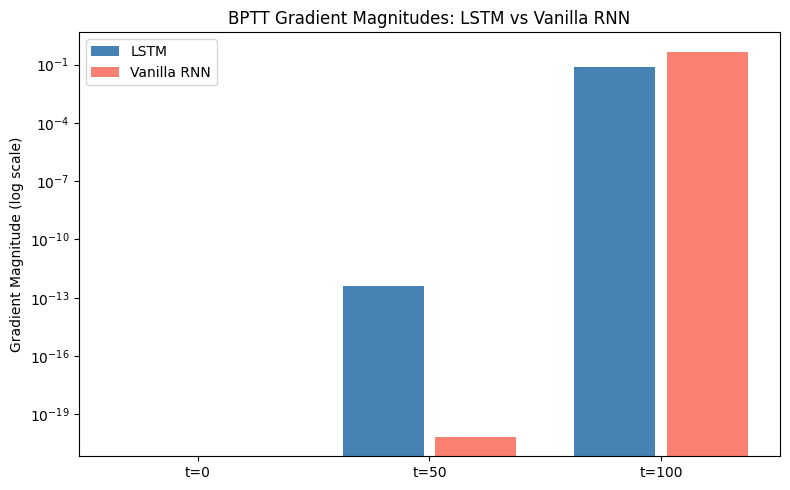
\includegraphics[width=0.48\linewidth]{q4_10_bptt_comparison.png}
  \caption{Comparsion of the gradient magnitude between RNN and LSTM.}
\end{figure}

The gradient at t = 50 remains much larger in LSTM than in the vanilla RNN.
\end{resultbox}

\subsection{4.11 GRU vs.\ LSTM Efficiency}
\vspace{6pt}
\begin{resultbox}
\begin{center}
\begin{tabular}{lccc}
\toprule
Model & Trainable parameters & Training time & Test MSE \\
\midrule
LSTM & 67,201 & 48.53 s & 0.9733 \\
GRU  & 50,433 & 81.35 s & 0.9702 \\
\bottomrule
\end{tabular}
\end{center}

% The best validation losses reported during training are $0.2452$ for the LSTM and $0.2432$ for the GRU.
\end{resultbox}

\subsection{4.12 Sequence-to-Sequence Forecasting}
\vspace{6pt}
\begin{resultbox}
Modified the LSTM to act as an Encoder-Decoder. The final test MSE is \textbf{0.6882}.

\begin{figure}[H]
  \centering
  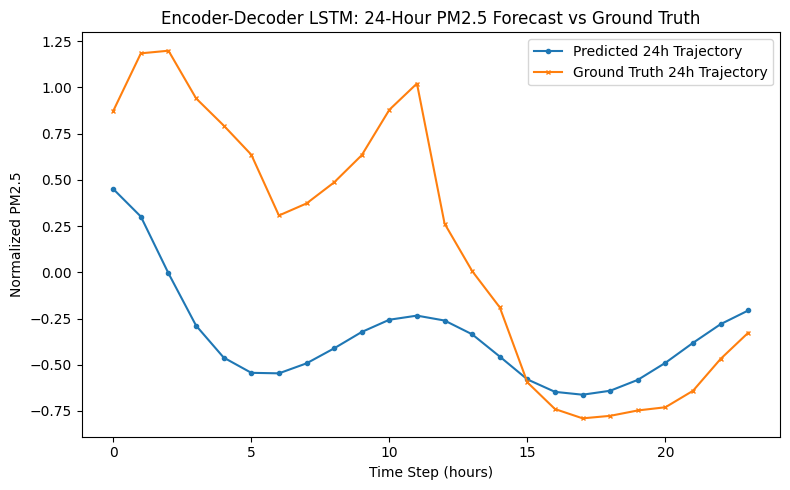
\includegraphics[width=0.5\linewidth]{q4_12_seq2seq_forecast.png}
  \caption{Model's 24-step prediction vs. ground truth.}
\end{figure}
\end{resultbox}

\section{Phase 5: Transformers \& Attention}

\subsection{5.13 Scaled Dot-Product Attention}
\vspace{6pt}
\begin{resultbox}
For tokens $Q,K,V \in \mathbb{R}^{T\times d}$, the scaled-dot product attention is computed as
\[
\mathrm{Attention}(Q,K,V)=\mathrm{softmax}\!\left(\frac{QK^\top}{\sqrt{d}}\right)V.
\]
% The output at the last time step is mapped to the scalar forecast. On the AQI task the best validation loss is \textbf{0.2468} and the test MSE is \textbf{1.1800}.

\begin{figure}[H]
  \centering
  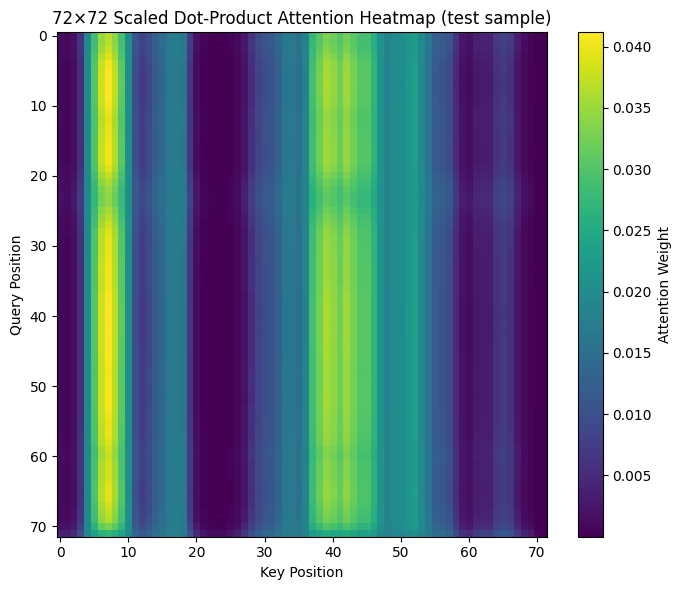
\includegraphics[width=0.42\linewidth]{q5_13_attention_heatmap.png}
  \caption{Attention map extracted for one AQI test sample.}
\end{figure}
\end{resultbox}


\subsection{5.14 The Necessity of Positional Encoding}
\vspace{6pt}
\begin{resultbox}
% The positional-encoding ablation uses the same single-head architecture, with and without sinusoidal encodings added to the token embeddings. The notebook records:
\begin{center}
\begin{tabular}{lcc}
\toprule
Model & Best validation loss & Test MSE \\
\midrule
Without positional encoding & 0.2517 & 1.3632 \\
With sinusoidal positional encoding & 0.2342 & 1.0986 \\
\bottomrule
\end{tabular}
\end{center}
% The accompanying derivation states the permutation-equivariant property
% \[
% \mathrm{Attention}(PX,PX,PX)=P\,\mathrm{Attention}(X,X,X),
% \]
% which is used in the notebook to explain the poorer performance without position information.
\end{resultbox}

\subsection{5.15 Vision Transformer (ViT)}
\begin{resultbox}
Each $128\times128$ segmented PlantVillage image is split into $16\times16$ non-overlapping patches, giving $64$ tokens per image, each of dimension $3\times16\times16=768$. The implemented ViT has \textbf{64,166} trainable parameters.

\begin{center}
\begin{tabular}{lccc}
\toprule
Model & Accuracy & Parameters & Parameter Efficiency (Accuracy / parameter) \\
\midrule
CNN (Phase 2) & 91.94\% & 2,113,262 & $4.35\times 10^{-7}$ \\
ViT (Phase 5) & 43.29\% & 64,166 & $6.75\times 10^{-6}$ \\
\bottomrule
\end{tabular}
\end{center}
\end{resultbox}

\section{Phase 6: Advanced Vision \& Imbalance}

\subsection{6.16 Transfer Learning \& Freezing}
\vspace{6pt}
\begin{resultbox}
A pretrained ResNet-18 backbone is loaded, the final classification head is modified to support 5 APTOS classes. All pretrained layers are frozen and only the final classification head is trained. Parameter counts for the model:
\[
\text{trainable} = 2{,}565,\qquad
\text{frozen} = 11{,}176{,}512,\qquad
\text{total} = 11{,}179{,}077.
\]
On the test split, the model achieves \textbf{77.45\%} accuracy.
% , \textbf{0.7947} quadratic weighted kappa, and cross-entropy loss \textbf{0.5753}.


\begin{figure}[H]
  \centering
  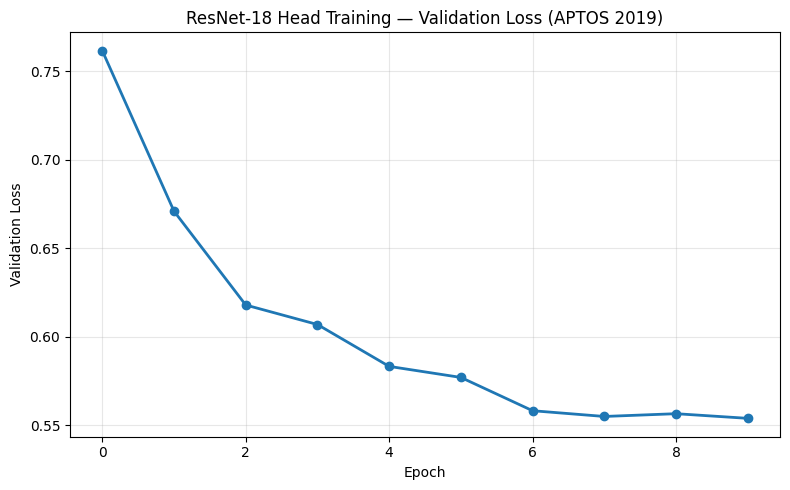
\includegraphics[width=0.49\linewidth]{q6_16_training_curve.png}
  \caption{Validation loss curve for the frozen-backbone ResNet-18.}
\end{figure}
\end{resultbox}

\subsection{6.17 Ordinal Imbalance & Focal Loss}
\vspace{6pt}
\begin{resultbox}
The focal-loss is implemented as 
\[
\mathcal{L}_{\mathrm{focal}} = -(1-p_t)^\gamma \log p_t,
\]
with $\gamma = 2.0$. Using the same pretrained ResNet-18 setup, the notebook reports:
\begin{center}
\begin{tabular}{lccc}
\toprule
Loss Type & Test loss & Accuracy & Cohen's Quadratic Weighted Kappa \\
\midrule
Cross-entropy & 0.5753 & 77.45\% & 0.7947 \\
Focal loss & 0.3159 & 77.45\% & 0.8138 \\
\bottomrule
\end{tabular}
\end{center}
The confusion matrices show that the evaluation is strongly class-imbalanced. The focal-loss model improves Cohen's Quadratic Weighted Kappa.
\end{resultbox}

\end{document}
